\documentclass{beamer}
\usepackage{moreverb} % Needed to allow comments, and verbatimwrite
\usepackage{verbatim}
\usepackage{ifthen} % Conditionals
\usepackage{bm} % BoldMath
\usepackage[econtex]{optional}

\usepackage[scale=2]{ccicons}
\usepackage{minted}
\usepackage{amsmath}
\usepackage{float}
\usepackage{setspace}
\usepackage{tikz}
\usepackage{caption}
\usemintedstyle{trac}
%\usepackage{biblatex}
%\addbibresource{economics.bib}

% if the line below is uncommented, bullets are shown step by step; comment out to make printable version
\beamerdefaultoverlayspecification{<+->}

% These are options to the compiler that can be sent at the command line
% This permits one document to generate multiple slightly different variations of the slides
\newboolean{WithOverlays}
\setboolean{WithOverlays}{true}
\newboolean{IMFMacroModelConf}
\setboolean{IMFMacroModelConf}{false}
%\setboolean{IMFMacroModelConf}{true}
\newboolean{FRBTalk}
\setboolean{FRBTalk}{false}
%\setboolean{FRBTalk}{true}
\newboolean{LSETalk}
\setboolean{LSETalk}{false}
\setboolean{LSETalk}{true}
\usepackage{optional}
\opt{NoOverlays}{\setboolean{WithOverlays}{false}\beamerdefaultoverlayspecification{}}

\mode<presentation>
{
  \usetheme{Warsaw}
  % or ...
  \setbeamercovered{transparent}
}

% Write the body to be read for autogeneration of printable version with 4 slides per page and no overlays
%\begin{verbatimwrite}{./HeteroMacro-Slides-body.tex} 
\opt{FromShell}{
\provideboolean{IMFMacroModelConf}
\setboolean{IMFMacroModelConf}{false}
\provideboolean{IMFMacroModelConf}
\setboolean{IMFMacroModelConf}{false}
\provideboolean{LSETalk}
\setboolean{LSETalk}{true}
\provideboolean{FRBTalk}
\setboolean{FRBTalk}{true}
}
\opt{IMFMacroModelConf}{\setboolean{IMFMacroModelConf}{true}}
\opt{LSETalk}{\setboolean{LSETalk}{true}}
\opt{FRBTalk}{\setboolean{FRBTalk}{true}}

\newcommand{\ifIMF}{\ifthenelse{\boolean{IMFMacroModelConf}}}
\newcommand{\ifFRB}{\ifthenelse{\boolean{FRBTalk}}}
\newcommand{\ifLSE}{\ifthenelse{\boolean{LSETalk}}}

\newboolean{HeteroMacro}
\setboolean{HeteroMacro}{true}

\usepackage{cancel}
\usepackage{econtexShortcuts}
%\newcommand{\newblock}{} % Needed to make beamer work with bibtex

\pdfmapfile{+sansmathaccent.map}
% Jirka's definitions
\usepackage{booktabs}
\usepackage{natbib}
%\usepackage{apalike}
\definecolor{jirkasred}{rgb}{0.9,0,0}
\newcommand{\jemph}[1]{{\color{jirkasred}#1}}
%\def\newblock{\hskip .11em plus .33em minus .07em}

\renewcommand{\ptyLev}{\ensuremath{Z}} % Z for productivity
\renewcommand{\urate}{\ensuremath{u}}
\renewcommand{\erate}{\ensuremath{\cancel{\urate}}}

%\setbeamertemplate{navigation symbols}{}  % Take away navigation symbols

%_____________ Opening slide _______________________

\title[HeteroMacro]{{Improving the Measurement \\ of Consumption Expenditure}}
\author[Carroll]{\scriptsize{Christopher Carroll\inst{1}}}

% - Use the \inst command only if there are several affiliations.
% - Keep it simple, no one is interested in your street address.
\institute{
  \inst{1} Johns Hopkins University and NBER\\   \texttt{ccarroll@jhu.edu} 
    }
\date{\today \\
\ifIMF{19th IMF Macro Modeling Conference \\ Armenia \\ September 2016}{}
\ifFRB{Presentation at Federal Reserve Board \\ September 2016 \\ Largely Based on \cite{cstwMPC} \\ {\small Thanks also to David Low, Nathan Palmer, and Alex Kaufman}}{}
\ifLSE{Panel Discussion at LSE Conference \\ ``New Perspectives on Consumption'' \\ December 2016}{}
}

\begin{document}

\begin{frame}[plain]
  \titlepage
\end{frame}

%\end{verbatimwrite}\opt{FromShell}{
\provideboolean{IMFMacroModelConf}
\setboolean{IMFMacroModelConf}{false}
\provideboolean{IMFMacroModelConf}
\setboolean{IMFMacroModelConf}{false}
\provideboolean{LSETalk}
\setboolean{LSETalk}{true}
\provideboolean{FRBTalk}
\setboolean{FRBTalk}{true}
}
\opt{IMFMacroModelConf}{\setboolean{IMFMacroModelConf}{true}}
\opt{LSETalk}{\setboolean{LSETalk}{true}}
\opt{FRBTalk}{\setboolean{FRBTalk}{true}}

\newcommand{\ifIMF}{\ifthenelse{\boolean{IMFMacroModelConf}}}
\newcommand{\ifFRB}{\ifthenelse{\boolean{FRBTalk}}}
\newcommand{\ifLSE}{\ifthenelse{\boolean{LSETalk}}}

\newboolean{HeteroMacro}
\setboolean{HeteroMacro}{true}

\usepackage{cancel}
\usepackage{econtexShortcuts}
%\newcommand{\newblock}{} % Needed to make beamer work with bibtex

\pdfmapfile{+sansmathaccent.map}
% Jirka's definitions
\usepackage{booktabs}
\usepackage{natbib}
%\usepackage{apalike}
\definecolor{jirkasred}{rgb}{0.9,0,0}
\newcommand{\jemph}[1]{{\color{jirkasred}#1}}
%\def\newblock{\hskip .11em plus .33em minus .07em}

\renewcommand{\ptyLev}{\ensuremath{Z}} % Z for productivity
\renewcommand{\urate}{\ensuremath{u}}
\renewcommand{\erate}{\ensuremath{\cancel{\urate}}}

%\setbeamertemplate{navigation symbols}{}  % Take away navigation symbols

%_____________ Opening slide _______________________

\title[HeteroMacro]{{New Perspectives on Consumption \\ Panel Discussion}}
\author[Carroll]{\scriptsize{Christopher Carroll\inst{1}}}

% - Use the \inst command only if there are several affiliations.
% - Keep it simple, no one is interested in your street address.
\institute{
  \inst{1} Johns Hopkins University and NBER\\   \texttt{ccarroll@jhu.edu}
    }
\date{\today \\
\ifIMF{19th IMF Macro Modeling Conference \\ Armenia \\ September 2016}{}
\ifFRB{Presentation at Federal Reserve Board \\ September 2016 \\ Largely Based on \cite{cstwMPC} \\ {\small Thanks also to David Low, Nathan Palmer, and Alex Kaufman}}{}
\ifLSE{London School of Economics \\ December 2016}{}
}

\begin{document}

\begin{frame}[plain]
  \titlepage
\end{frame}


\begin{frame}\frametitle{Progress!}

\pause
\bi
\item I feel the way Galileo must have felt ...
\item ... before he started grinding lenses
\item Conference shows lots of people grinding away!
\bi
\item National Registry Data (`Registries')
\item Administrative Data from Aggregators (`Aggregators')
\item Consumer Credit Panels (`CCP')
\item Surveys
\ei

\ei


\end{frame}

\begin{frame}\frametitle{What Would the Perfect Lens Look Like?}

Perfection:
\bi
\item Huge Sample Sizes
\bi
\item (Registries; Aggregators)
\ei
\item Accurately Measured Data on $\cRat, \yRat, \aRat, \dRat$
\bi
\item (Registries; Aggregators)
\ei
\item Data on {\it expectations} and {\it preferences}
\bi
\item (Surveys)
\ei
\ei

What we most desperately need:
\bi
\item  {\it Integrated}: Balance sheets {\it and} expectations
\item Leth-Petersen is the only example (and small sample size)
\ei

\end{frame}


% \section{Why Do We Care?}
\begin{frame}\frametitle{Why Do We Care?}

\bi
\item Microeconomics
\bi
\item Lots of reasons
\ei
\item Macroeconomics
\bi
\item ``Aggregate Demand''
%\item Capital Stock $\Rightarrow$ Interest Rates
\item Finance-Macro Nexus
\ei
\ei

\end{frame}

\begin{frame}\frametitle{Larry Summers' Infamous Quote about 2009-10}

{\it ``Almost nothing from the academic macroeconomics literature over the prior
30 years was useful in understanding what to do''}


\begin{center}
\phantom{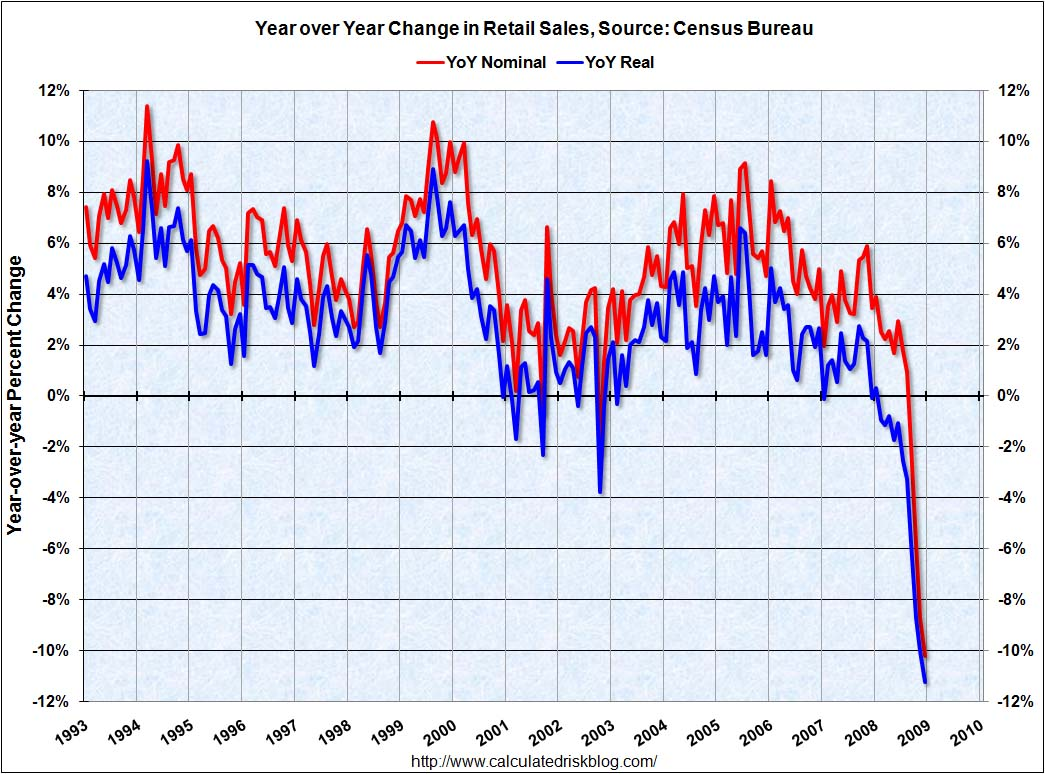
\includegraphics[width=2.5in]{/Volumes/Data/Job/Discuss/DiMaggio_Kermani/LaTeX/cfpbpresentation/Figures/Retail-Sales-Collapse.jpg}}
\end{center}

\end{frame}


\begin{frame}\frametitle{The Holy Grail}

\bi
\item A {\it reliable} (set of) {\it quantitatively useful} structural models
\bi
\item Theorists can
\ei
\item What do we need?
\bi
\item Much better {\it data and  {\bf models}} of expectations
\item Measures of {\it behavior conditional on expectations} ...
\item ... to be fed into a calibrated strucutural model
\ei
\ei

\end{frame}

\begin{frame}\frametitle{Wealth Effects (`Nexus')?}
\bi
\item ``Housing Wealth Effect'' estimates are converging
\item Kaplan, Mitman, Violante; Leth-Petersen and Andersen; CKHI
\item {\it Crucial} point: Size of effect depends on credit availability (`collateral channel')
\ei
\end{frame}


\begin{frame}\frametitle{Larry Summers' Infamous Quote about 2009-10}

{\it ``Almost nothing from the academic macroeconomics literature over the prior
30 years was useful in understanding what to do''}

\begin{center}
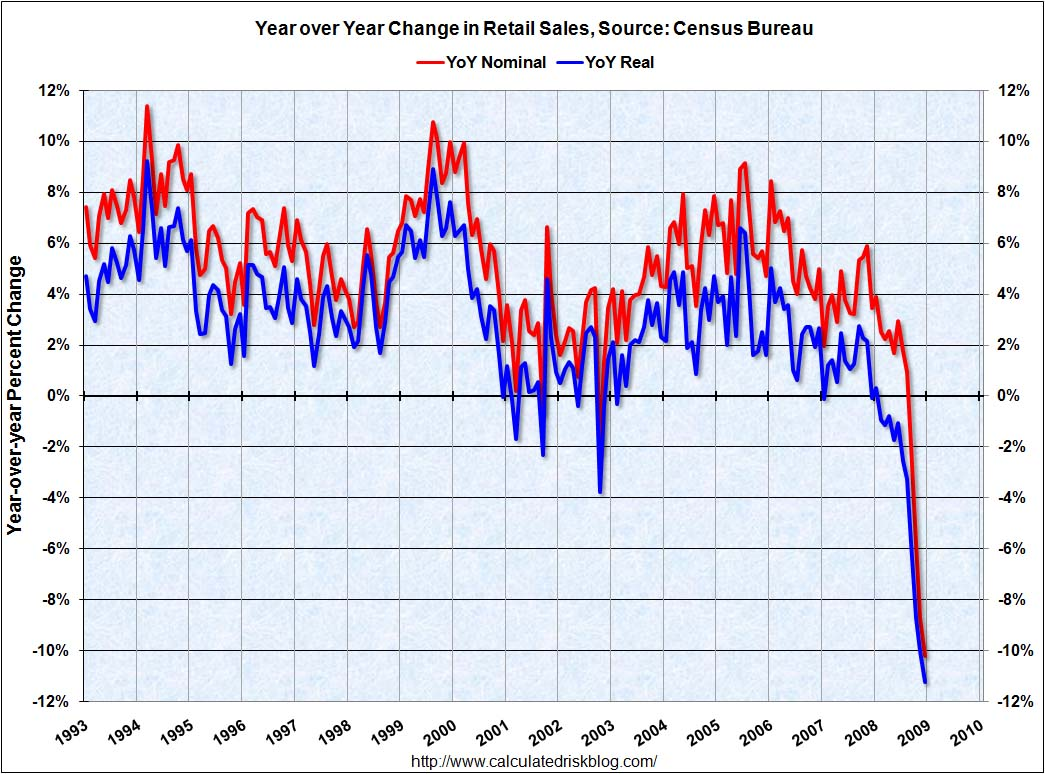
\includegraphics[width=2.5in]{/Volumes/Data/Job/Discuss/DiMaggio_Kermani/LaTeX/cfpbpresentation/Figures/Retail-Sales-Collapse.jpg}
\end{center}

\end{frame}

\begin{frame}\frametitle{Off-the-shelf Macro Models}

Zombies:
\bi
\item Rep Agent/Certainty Equivalent DSGE models
\item Campbell-Mankiw (Savers/Spenders)
\ei

Desiderata: Uncertainty and Heterogeneity
\bi
\item Uncertainty
\bi
\item Landais \& Spinnewijn: Unemployment $\Rightarrow$ $C \downarrow$
\item $\Rightarrow$ uncertainty is hugely important
\ei
\item Heterogeneity
\bi
\item Concavity of the Consumption Function:
\bi
\item Low wealth people have much higher MPC's
\ei
\ei
\ei



\end{frame}

\begin{frame}\frametitle{Saving Over the Business Cycle}
\begin{center}
\includegraphics[width=3.0in]{/Volumes/Data/Papers/cssUSSaving/Latest/Figures/saving.pdf}
\end{center}
\end{frame}

\begin{frame}\frametitle{Unemployment Expectations $\Ex[\Delta \uLev_{t+1}]$}
\begin{center}
\includegraphics[width=3.0in]{/Volumes/Data/Papers/cssUSSaving/Latest/Figures/fUExp.pdf}
\end{center}
\end{frame}


\begin{frame}\frametitle{\cite{cssUSSaving}}

Model fit to aggregate saving rate history fits well.  Ranking of reasons for $s$ rise: \pause
\begin{itemize}
\item 60 percent: Uncertainty
\bi
\item Michigan Survey: Unemployment Expectations
\ei
\item 25 percent: Wealth Effects
\item 15 percent: Credit Supply
\end{itemize}

\end{frame}

\begin{frame}\frametitle{National Registry Data}

Most important question they can answer:
\bi
\item {\it Whose} circumstances ($\yRat$, $\aRat$, etc) change
\item Whose {\it behavior} changes (`active saving')
\bi
\item Regional differences will be profoundly useful
\ei
\ei

\end{frame}

\begin{frame}\frametitle{High Frequency Data (Shapiro; Schuh)}

{\bf More is different:}
\bi
\item {\it Everything} is durable at the weekly frequency
\item Expenditure shocks can't be ignored
\item More `coping strategies' than we usually model
\ei

\end{frame}

\begin{frame}\frametitle{Surveys}

\begin{enumerate}
\item Survey design
\bi
\item Transaction, wealth, income data
\bi
\item Collect using technology (\texttt{Mint.com}, other aggregators)
\ei
\item Only survey people on beliefs, expectations, preferences
\ei
\item Use admin data as sampling frame for surveys
\bi
\item That way you get the combination
\ei
\bi
\item Need panel data on expectations to model them
\ei
\end{enumerate}

\end{frame}

\begin{frame}\frametitle{A New Day Is Dawning! }

\pause
The scientific revolution is coming to macroeconomics!


\end{frame}


 
%\end{document}

\section{Benchmark Model}

\begin{frame}
In a model with `serious' household heterogeneity (`HH'):\pause
\begin{enumerate}
\item Fiscal Policy Can Be Much More Powerful than in RA model
\begin{itemize}
\item \ifIMF{$\Rightarrow$ austerity has much bigger medium-term effects}{}\ifFRB{But stimulative effect depends {\it completely} on details \bi \item Who Gets \$ \item When do they get it \ei }{}
\end{itemize}
\item Monetary Policy Mechanism Is Radically Different
\begin{itemize}
\item Effect of $\rfree$ mostly {\it not} about intertemporal substitution
\item QE works when it affects people with high MPC; otherwise, not
\end{itemize}
\item Changes in {\it micro} Uncertainty Can Matter A Lot
\begin{itemize}
\item When Michigan $\Ex_{t}[\Delta U_{t+1}] \uparrow$, $C \downarrow$
\item Explains Why Saving Rate $\uparrow$ in Recessions
\end{itemize}
\item New Tools $\Rightarrow$ It's Not As Hard As You Think!
\begin{itemize}
\item {\bf A}lgorithmic {\bf R}esources and tool{\bf K}it: {\bf ARK!}
\item Initiative of U.S.\ Consumer Financial Protection Bureau
\item Subset: {\bf H}eterogeneous {\bf A}gents {\bf R}esources and tool{\bf K}it:
\item[] ~~~~~~~~~~\href{http://econ-ark.org}{\jemph{http://econ-ark.org}}
\end{itemize}
\end{enumerate}
\end{frame}

%\begin{frame}\frametitle{{\bf N}ot {\bf O}nly {\bf A}bout {\bf H}eterogeneous-agent {\bf s}olutions}

%\phantom{{\Large NOAHs-ARK!}}
%\end{frame}

%\begin{frame}\frametitle{{\bf N}ot {\bf O}nly {\bf A}bout {\bf H}eterogeneous-agent {\bf s}olutions}

%{\Large NOAHs-ARK!}
%\end{frame}

\subsection{The Key is Getting {\it Micro} Consumption Right}
\subsubsection{The MPC}

\begin{frame}\frametitle{Household Heterogeneity and Aggregate Consumption}

\begin{block}{Key Question: How Large Is \textbf{`the MPC'} $(\equiv \MPC)$?}
If households receive a surprise extra 1 unit of income,\\ how much will be spent over the next year?
\end{block}

\begin{block}{Elements that interact to produce the answer:}
\bi
\item Households are heterogeneous {\it ex post} and {\it ex ante}
\item Lots of HH's who do lots of $C$ have little wealth
\item $\cFunc$ function is highly concave
\item $\Rightarrow$ Distributional issues matter for aggregate C\\
Giving 1 to the poor $\ne$ giving 1 to the rich
\ei
\end{block}

\end{frame}



%_______________________________________
%\begin{frame}[label=AIMCB]
%\frametitle{Our Claim: Heterogeneity Is Key To Modeling the MPC}

%\begin{itemize} \pause
%\begin{itemize}
%\item \citet{claridaMeaCulpa}: Missing this is why DSGE models failed
%\end{itemize}
%  \item Why might heterogeneity matter?
    %\begin{itemize}
  %    \item People with different income expectations behave differently
%      \item Theory: HH $\cFunc$ function is {\it concave} in market resources $\mRat$
%      \begin{itemize}
%        \item HH's at different $m~\rightarrow$ {\it optimally} behave very differently
%        \item In addition to the MPC, $\mRat$ affects
% \begin{itemize}
%        \item  $L$ supply (``paradox of toil'')
%        \item risk aversion of the value function
%        \item response to financial shocks (say, revised view of $\sigma^{2}_{\text{stocks}}$)
%     \end{itemize}
%    \end{itemize}

%\end{itemize}
%\end{frame}




\subsubsection{Theory and Evidence}
\begin{frame}[label=cFuncAndW]
\frametitle{Consumption Concavity and Wealth Heterogeneity}
\begin{figure}
\centering
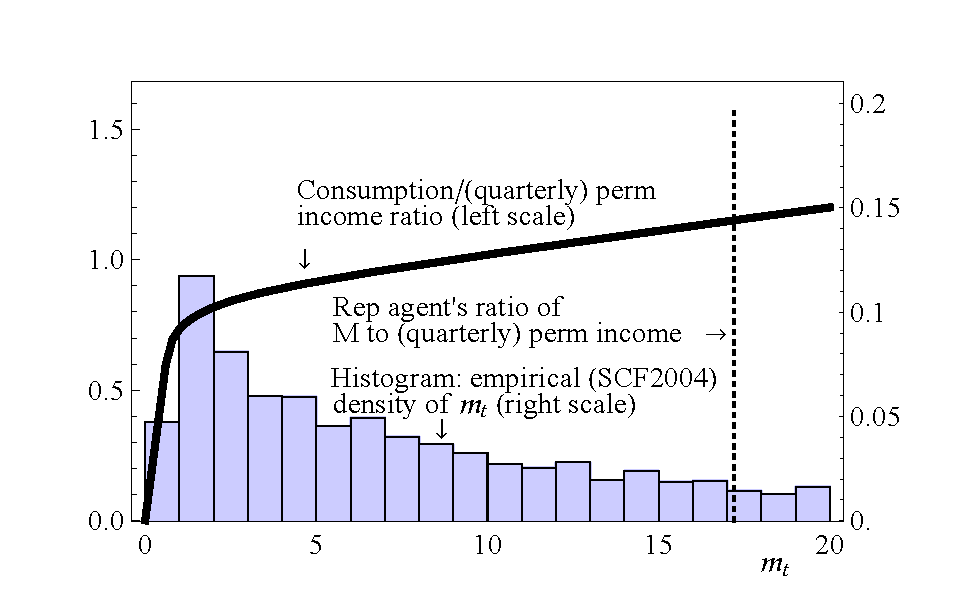
\includegraphics[width=\textwidth,height=6.3cm]{../Figures/CFuncPointAndHistNetWorthRepLinePlot.pdf}
\end{figure}
\end{frame}




\begin{frame}
\frametitle{{To-Do List}}


\begin{enumerate}
\item Calibrate realistic HH income process:
\bi
\item Match micro income {\it dynamics} and cross-section distribution
\ei 
\item Match empirical wealth distribution
\item Back out optimal $\cFunc$ and $\cFunc^{\prime}(\mRat)=\MPC(\mRat)$ out of transitory income
\item Is MPC in line with empirical estimates?
\end{enumerate}

%\ifthenelse{\boolean{HeteroMacro}}{\begin{comment}}{}
%\begin{block}{Our Question:}
%\jemph{Does a model that matches micro facts} about income dynamics and wealth distribution \jemph{give different} (and more plausible) \jemph{answers} than KS \jemph{to macroeconomic questions} (say, about the response of consumption to fiscal `stimulus')?
%\end{block}
%\ifthenelse{\boolean{HeteroMacro}}{\end{comment}}{}

\end{frame}

\ifthenelse{\boolean{HeteroMacro}}{}{\import ./Individual/FriedmanPIH.tex}

\subsection{Model Without Aggregate Shock}

\subsubsection{Income Process}
\begin{frame}
\frametitle{{Our (Micro) Income Process}}

Idiosyncratic (household) income process is logarithmic Friedman:
  \begin{eqnarray*}
\yLev_{t+1}&=&\pRat_{t+1}\tshk_{t+1}\Wage\\
\pRat_{t+1}&=&\pRat_{t}\pshk_{t+1}
\end{eqnarray*}
\begin{center}
\begin{tabular}{rcl}
$\pRat_{t}$ & - & permanent income\\
$\psi_{t+1}$ & - & permanent income\\
$\Ex_{t}[\tshk_{t+n}]=1$ & - & transitory income\\
$\Ex_{t}[\pshk_{t+n}]=1$ & - & permanent shock\\
$\Wage$ & - & aggregate wage rate
\end{tabular}
\end{center}

Generates {\it ex post} dist'n of $\yRat$ that matches cross-section data

\end{frame}


\begin{frame}
\frametitle{Unemployment and Unemployment Insurance}

\begin{block}{Modifications from \citet{carroll:brookings}}
Transitory income $\tshk_{t}$ incorporates \jemph{unemployment insurance}:
\begin{eqnarray*}
\tshk_{t} &=&\mu \text{ with probability $u$} \\
&=&(1-\tau)\bar{\ell}\theta_{t}\text{ with probability $1-u$}
\end{eqnarray*}
$\mu$ is UI when unemployed\\
 $\tau$ is the rate of tax collected for the unemployment benefits
\end{block}

\end{frame}


%_______________________________________
\subsubsection{Decision Problem}
\begin{frame}
\frametitle{{Model Without Aggr Uncertainty: Decision Problem}}

\providecommand{\uFunc}{\mathrm{u}}

\begin{eqnarray*}
\valfn(\mRat_{t})&=& \underset{\{\cFunc_{t}\}}{\max } ~~
\uFunc(\cRat_{t})
+\Discount \PLives \Ex_{t}\left[ \pshk_{t+1}^{1-\CRRA}\valfn(\mRat_{t+1})
\right]   \label{eq:hetdecisionprobnashk}\\
\notag &\text{s.t.}&\\
\notag \wEndRat_{t} &=&\mRat_{t}-\cRat_{t} \\
\notag \wEndRat_{t} &\geq &0 \\
\kRat_{t+1} &=&\wEndRat_{t}/(\PLives \pshk_{t+1})  \label{indconst3}
\\
\mRat_{t+1} &=&(\daleth +\rProd)\kRat_{t+1}+\tshk_{t+1} \label{indconst4} \\
\notag \rProd &=&\kapShare\ptyLev(\KLev/\bar{\ell}\LLev)^{\kapShare-1}
\end{eqnarray*}
(State and control variables normalized by $\pRat_{t} \Wage$)

\end{frame}


%_______________________________________
%\subsubsection{What Happens After Death?}
\subsubsection{There Is an Ergodic Distribution of Permanent Income}
\begin{frame}
\frametitle{{What Happens After Death?}}

\pause
\begin{itemize}
\item You are replaced by a new agent whose permanent income $\pRat$ is equal to the population mean
\item Prevents dist'n of $\pRat$ from spreading out, so long as
\item[] $$\PLives \Ex[\pshk^{2}] < 1$$
\item[] which holds for our parameterization (next slide)
\end{itemize}
\end{frame}


%_______________________________________
%\subsubsection{There Is an Ergodic Distribution of Permanent Income}
%\begin{frame}
%\frametitle{{$\exists$ Ergodic Distribution of Permanent Income}}
%
%Exists, if death eliminates permanent shocks:
%$$\PLives \Ex[\pshk^{2}] < 1.$$
% \jemph{Holds.}\\[5mm]
%Population mean of $\pRat^{2}$:
%\begin{eqnarray}
%\Mean[\pRat^{2}] & = & \frac{\PDies}{1-\PLives\Ex[\pshk^{2}]}\notag
%\end{eqnarray}
%
%\end{frame}
%
%_______________________________________
\subsubsection{Parameter Values}
\begin{frame}
\frametitle{{Parameter Values}}
\begin{itemize}
  \item $\beta $, $\CRRA $, $\kapShare $, $\delta $, $\bar{\ell}$, $\mu$ , and $\uFunc$ taken from JEDC special volume %(from \citet{denhann:comp})
  \item Main new parameter values:
\end{itemize}

  \begin{footnotesize}
  \begin{table}
  %\caption{Parameter Values}

  \begin{center}
  \begin{tabular}{cccc}
  \toprule
  Description              & Param       & Value   & Source\\ \midrule
  Prob of Death per Quarter& $\PDies$        & $0.00625$ & Life span of 40 years\\
  Variance of Log $\pshk_{t}$ & $\sigma _{\pshk}^{2}$ & $0.016*4/11$ &\text{\small{\citet{carroll:brookings}}}; SCF \\
    & & & \text{\small{DeBacker et al.\ (2013)}}\\
  Variance of Log $\theta _{t}$ & $\sigma _{\theta }^{2}$& $0.010\times 4$ & \text{\small{\citet{carroll:brookings}}}\\
 \bottomrule
  \end{tabular}
  \end{center}
  \end{table}
  \end{footnotesize}

\end{frame}



%_______________________________________
%\subsubsection{Annual Income Variances}
%\begin{frame}
%\frametitle{{Annual Income, Earnings, or Wage Variances}}
%
%\begin{tiny}
%\input ../Tables/EstimatesOfVarsslides.tex
%
%\tiny{$^{\star}$\citet{meghir&pistaferri} and \citet{bppInequality} assume that the transitory component is serially correlated (an MA process), and report the variance of a subelement of the transitory component. $\sigma_{\tshk}^{2}$ for these articles are calculated using their MA estimates. }
%\end{tiny}
%
%\end{frame}
%
%
%
%\subsubsection{Estimation/Results}


%_______________________________________
\subsubsection{Our Strategy}
%\begin{frame}
%\frametitle{{Our Strategy}}
%\begin{enumerate}
%  \item Estimate the time preference factor $\beta$ without aggregate shock
%  \item Using estimated $\beta$, run model(s) with aggregate shocks
%\end{enumerate}
%\end{frame}



\begin{frame}
\frametitle{{Variants of Our Model---{Four Dimensions}}}

\begin{block}{}\footnotesize
\begin{enumerate}
\item \jemph{Discount Factor $\Discount$}
\bi \scriptsize
\item \jemph{`$\Discount$-Point' model:} Single discount factor
\item \jemph{`$\Discount$-Dist' model:} Uniformly distributed discount factor
\ei
\item \jemph{Aggregate Shocks}
\bi \scriptsize
\item (No)
\item Krusell--Smith
\item Friedman/Buffer Stock
\ei
\item \jemph{Empirical Wealth Variable to Match}
\bi \scriptsize
\item Net Worth
\item Liquid Financial Assets
\ei
\item \jemph{Life Cycle}
\bi \scriptsize
\item Perpetual Youth ({\it a la} Blanchard)
\item Overlapping Generations
\ei
\end{enumerate}
\end{block}

\end{frame}


\begin{frame}
\frametitle{Estimation of $\Discount$-Point and $\Discount$-Dist}

\begin{footnotesize}
\begin{block}{`$\Discount$-Point' model}
\bi
\item `Estimate' single $\grave{\Discount}$ by matching the capital--output ratio
\ei
\end{block}
\begin{block}{`$\Discount$-Dist' model---Heterogenous Impatience}
\begin{itemize}
\item Assume uniformly distributed $\Discount$ across households
%\item Estimate the band $[\grave{\Discount}-\nabla,\grave{\Discount}+\nabla]$ by matching net worth held by the top 20, 40, 60, 80\%
\item Estimate the band $[\grave{\Discount}-\nabla,\grave{\Discount}+\nabla]$ by \jemph{minimizing distance between model ($w$) and data ($\omega$) net worth} held by the top 20, 40, 60, 80\%
%        \item The uniform distribution is approximated by 7 points
       % \item \jemph{Minimize distance b/w model ($w$) and data ($\omega$) wealth quantiles}:
        \begin{equation*}
        \underset{\{\grave{\Discount}, \nabla\}}{\min}\sum\limits_{i=20,40,60,80}(w_{i}-\omega _{i})^{2}\notag,
        \end{equation*}
        s.t. aggregate net worth--output ratio matches the steady-state value from the perfect foresight model\\[2mm]
        %\footnotesize $w_{i}$ and $\omega _{i}$ are proportions of net worth held by the top $i$ percent in our model and in the data, respectively
\end{itemize}
\end{block}
\end{footnotesize}

\end{frame}

\begin{frame}\frametitle{Alternatives to $\Discount$ Heterogeneity}

Perfect foresight `impatience' condition is:

\begin{eqnarray}
  \left(\frac{(\Discount \Rfree \PLives)^{1/\CRRA}}{\PGro}\right) & < & 1
\end{eqnarray}

Behavior will depend on {\it degree} of impatience: 1-$\left(\frac{(\Discount \Rfree \PLives)^{1/\CRRA}}{\PGro}\right)$

Point:  Hetero in {\it beliefs}
\begin{itemize}
\item In PF model, about ${\PGro,\Rfree,\PLives}$ generate {\it identcal} consequences
\item In model with uncertainty, even more options:
\bi 
\item hetero. in {\it beliefs} about $\sigma^{2}_{\psi}$ and $\sigma^{2}_{\theta}$ and $\mu$)
\ei
\end{itemize}



\end{frame}
%_______________________________________

\begin{frame}
\frametitle{{Results: Wealth Distribution}}

\begin{figure}
\centering
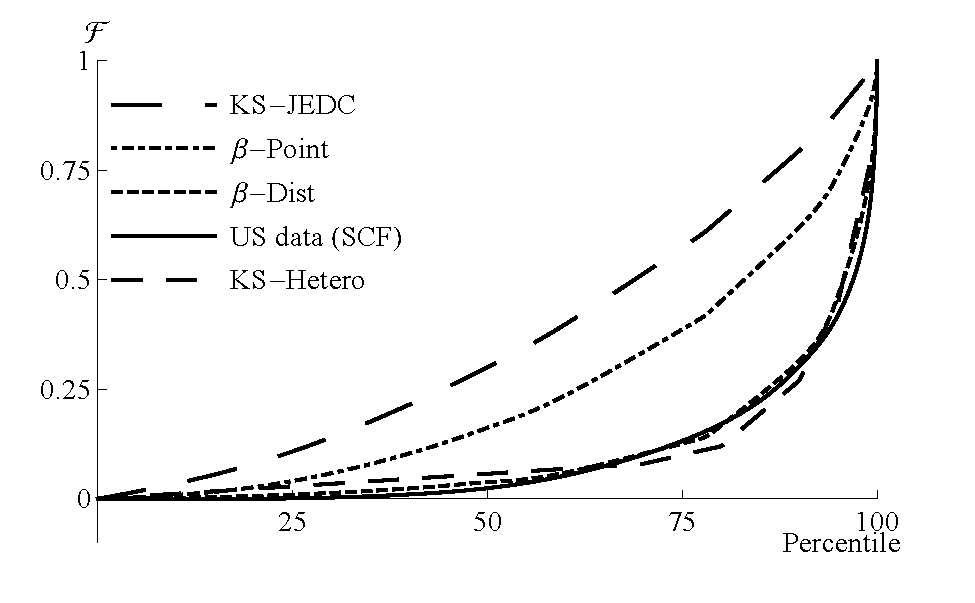
\includegraphics[width=0.9\textwidth]{../Figures/CumWLevSCFCastanedaAndDistSevenNoAggShockPlot.pdf}
%\caption{Cumulative Distribution of Net Worth}
\label{CumWLevSCFCastanedaAndDistSevenNoAggShockPlot}
\end{figure}

\end{frame}



\begin{frame}
\frametitle{{Results: Wealth Distribution}}

\begin{table}
\begin{footnotesize}

\input ../Tables/WDistslides.tex

\end{footnotesize}
\end{table}
\tiny{Notes: $^{\ddagger}:$ $\grave{\Discount}=
\input ../../../cstCode/Latest/Code/Mathematica/Results/Beta.tex
$.
$^{\star}:$ $(\grave{\Discount}, \nabla)=(
\input ../../../cstCode/Latest/Code/Mathematica/Results/Betamiddle.tex
,
\input ../../../cstCode/Latest/Code/Mathematica/Results/nabla.tex
)$%
.
Bold points are targeted. $\KLev_{t}/\YLev_{t}=10.3$. }
\end{frame}

%_______________________________________
\subsubsection{Results: Marginal Propensity to Consume}

\begin{frame}
\frametitle{{Marginal Propensity to Consume and Net Worth}}

\begin{figure}
\centering
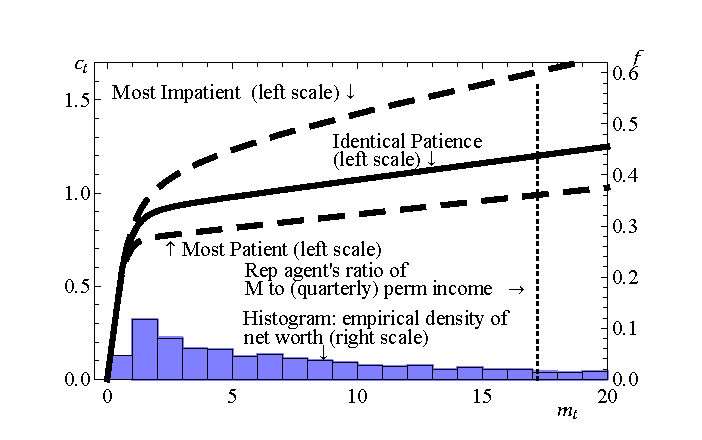
\includegraphics[width=\textwidth,height=6cm]{../Figures/CFuncDistSevenPointPermAndHistNetWorthPlotFedQuarterly.pdf}
\end{figure}

\end{frame}

\begin{frame}
\frametitle{{Empirical Estimates of MPC: $\boldsymbol{\sim}$0.2--0.6}}
\centerline{\cite{friedman:windfalls} estimated $\MPC = 1/3$}

\begin{tiny}
%\begin{table}
\input ../Tables/mpcLitSlides.tex
%\end{table}
\tiny{Notes: $^{\ddagger}$: elasticity.}
\end{tiny}

\end{frame}

%_______________________________________
\begin{frame}
\frametitle{{Model Results: MPC (in Annual Terms)}}
\begin{tiny}
\begin{table}
\input ../Tables/MPCslides.tex
\end{table}
\tiny{Notes: Annual MPC is calculated by $1-(1-$\text{quarterly MPC}$)^{4}$.
% See the paper for a discussion of the extensive literature that generally estimates empirical MPC's in the range of 0.3--0.6.
}
\end{tiny}
\end{frame}

%_______________________________________


\begin{frame}
\frametitle{{Typology of Our Models---{Four Dimensions}}}

\begin{block}{}\footnotesize
\begin{enumerate}
\item<0-0> \jemph{Discount Factor $\Discount$}
\bi \scriptsize
\item \jemph{`$\Discount$-Point' model:} Single discount factor
\item \jemph{`$\Discount$-Dist' model:} Uniformly distributed discount factor
\ei
\item<1-> \jemph{Aggregate Shocks}
\bi \scriptsize
\item (No)
\item Krusell--Smith
\item Friedman/Buffer Stock
\ei
\item<0-0> \jemph{Empirical Wealth Variable to Match}
\bi \scriptsize
\item Net Worth
\item Liquid Financial Assets
\ei
\item<0-0> \jemph{Life Cycle}
\bi \scriptsize
\item Perpetual Youth (a la Blanchard)
\item Overlapping Generations
\ei
\end{enumerate}
\end{block}

\end{frame}




\begin{frame}
\frametitle{{Results: MPC Is Stable Over the Business Cycle}}
There Is Such a Thing as `the MPC':
\begin{tiny}
\begin{table}
\input ../Tables/MPCoverBCslides.tex
\end{table}
\end{tiny}
\end{frame}



\begin{frame}
\frametitle{{Typology of Our Models---{Four Dimensions}}}

\begin{block}{}\footnotesize
\begin{enumerate}
\item<0-0> \jemph{Discount Factor $\Discount$}
\bi \scriptsize
\item \jemph{`$\Discount$-Point' model:} Single discount factor
\item \jemph{`$\Discount$-Dist' model:} Uniformly distributed discount factor
\ei
\item<0-0> \jemph{Aggregate Shocks}
\bi \scriptsize
\item (No)
\item Krusell--Smith
\item Friedman/Buffer Stock
\ei
\item<1-> \jemph{Empirical Wealth Variable to Match}
\bi \scriptsize
\item Net Worth
\item Liquid Financial Assets
\ei
\item<0-0> \jemph{Life Cycle}
\bi \scriptsize
\item Perpetual Youth (a la Blanchard)
\item Overlapping Generations
\ei
\end{enumerate}
\end{block}

\end{frame}

\subsection{Matching Net Worth vs Liquid Assets}
\subsubsection{Net Worth vs Liquid Assets}
\begin{frame}[label=cfuncVsLiq]
\frametitle{Dimension 3: Matching Net Worth vs.\ Liquid Assets}
\begin{figure}
\centering
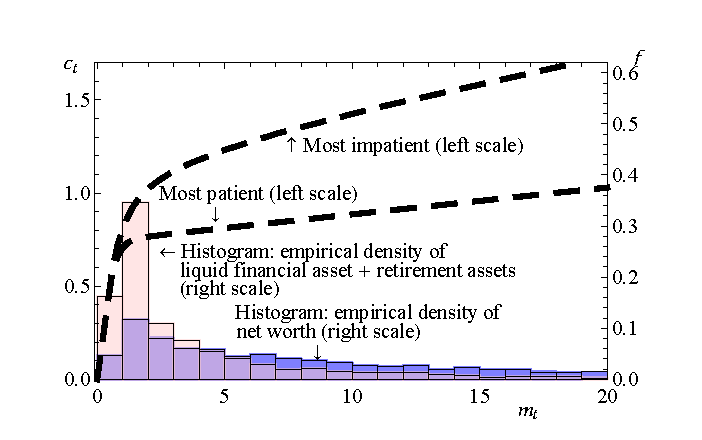
\includegraphics[width=0.8\textwidth]{../Figures/CFuncDistSevenPermAndHistNetWorthLiqFinPlsRetPlot.pdf}
\end{figure}
{\footnotesize Liquid Assets $\equiv$ transaction accounts,
CDs, bonds, stocks, mutual funds}
\end{frame}


%_______________________________________
\begin{frame}
\frametitle{{Match Net Worth vs.\ Liquid Financial Assets
%\\
%MPC: 0.19 $\uparrow$ 0.68
}}

\begin{itemize}
  \item Buffer stock saving driven by accumulation of \jemph{liquidity}
  \item May make more sense to match liquid (and retirement) assets\\ (\citet{hall:slump}, \citet{kvStim})
  \item \jemph{Aggregate MPC Increases Substantially: 0.23 $\uparrow$ 0.44}
\end{itemize}

\begin{footnotesize}
\begin{table}
\input ../Tables/MPCslidesLiqFinPlsRet.tex
\end{table}
\tiny{Notes: Annual MPC is calculated by $1-(1-$\text{quarterly MPC}$)^{4}$.}
\end{footnotesize}

\end{frame}





\begin{frame}[label=cfunc]
\frametitle{{Distribution of MPCs}}

{\jemph{Wealth heterogeneity translates into heterogeneity in MPCs}}

\begin{figure}
\centering
% 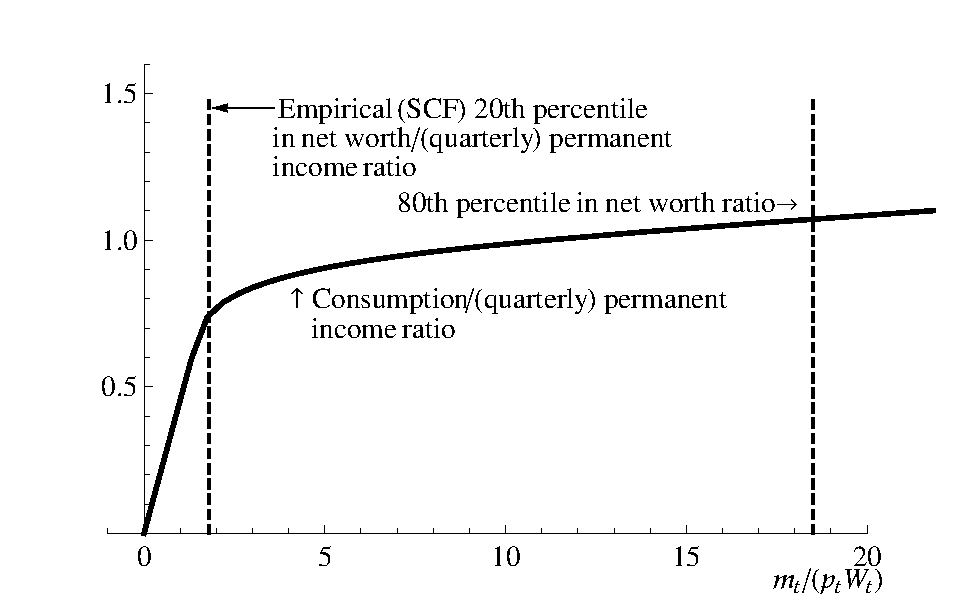
\includegraphics[width=\textwidth]{../Figures/CFuncPointPlotNW2080.pdf}
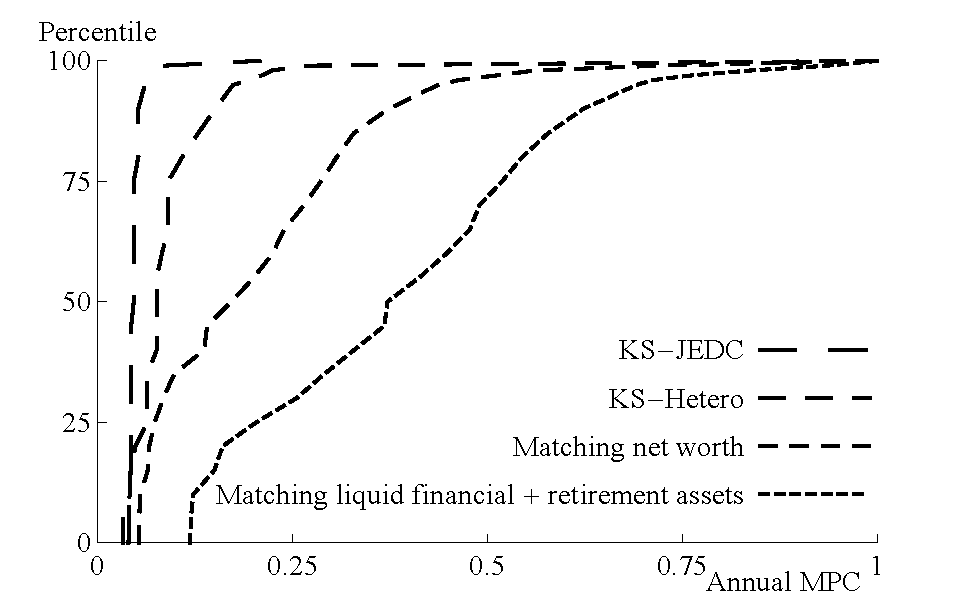
\includegraphics[width=0.8\textwidth]{../Figures/DistributionsMPCsDistSevenAndKSKSAggShocksPlot.pdf}

\end{figure}

\end{frame}



\subsection{Life Cycle Model}
\subsubsection{Overlapping Generations}
\begin{frame}
\frametitle{Dimension 4: Overlapping Generations}
\jemph{\textbf{Realistic Life-Cycle Model}}
\bi
\item Three education levels: $e\in\{D, HS, C\}$
\item Age/education-specific income profiles
\begin{eqnarray*}
\yLev_t &=& \tshk_t \pLev_t = (1 - \tau)\theta_t \pLev_t,\\
\pLev_t &=& \pshk_t \overline{\pshk}_{es} \pLev_{t-1}
\end{eqnarray*}
\bi
\item Age-specific variances of income shocks
\item Transitory unemployment shock with prob $\urate$
\ei
\item Household-specific mortality $\PDies_{es}$
\ei
\end{frame}

\subsubsection{Household Decision Problem}

\begin{frame}
\frametitle{Household Decision Problem}
\begin{eqnarray*}
\vFunc_{es}(\mRat_t) &=& \max_{\cRat_t} \uFunc(\cRat_t) + \Discount \PLives_{es} \Ex_t \left[\pshk_{t+1}^{1-\CRRA} \vFunc_{es+1}(\mRat_{t+1})\right]\\
\notag &\text{s.t.}&\\
\aRat_t &=& \mRat_t - \cRat_t,\\
\kRat_{t+1} &=& \aRat_t/\pshk_{t+1},\\
\mRat_{t+1} &=& (\daleth +\rProd) \kRat_{t+1} + \tshk_{t+1},\\
\aRat_t &\geq& 0
\end{eqnarray*}
\end{frame}

\subsubsection{Macro Dynamics}
\begin{frame}
\frametitle{Macro Dynamics}
\bi
\item Population growth $N$, technological progress $\Gamma$
\item \jemph{Tax rate} to finance social security and unemployment benefits: $\tau=\tau_{SS}+\tau_U$
\item
$
\tau_{SS} = \frac{\sum_{e \in \{D,HS,C\}} \Big[ \theta_e \overline{\pLev}_{e0} \sum_{t = 164}^{384} \big( ((1 + \Gamma)(1+N))^{-t} \prod_{s=0}^t ( \overline{\pshk}_{es} \PLives_{es} ) \big) \Big]}
{\sum_{e \in \{D,HS,C\}} \Big[ \theta_e \overline{\pLev}_{e0} \sum_{t = 0}^{163} \big( ((1 + \Gamma)(1+N) )^{-t} \prod_{s=0}^t ( \overline{\pshk}_{es} \PLives_{es} ) \big) \Big]}
$
\item $\tau_U=\urate\mu$
\ei
\end{frame}

\subsubsection{Calibration}
\begin{frame}
\frametitle{Calibration}

\begin{table}
\footnotesize
\label{table:ParametersLifeCycle}
\begin{center}
\begin{tabular}{l c c}
\toprule
Description & Parameter & Value \\
\midrule
Coefficient of relative risk aversion & \CRRA & 1 \\
Effective interest rate & $(\rProd - \delta)$ & 0.01 \\
Population growth rate & $N$ & 0.0025 \\
Technological growth rate & $\Gamma$ & 0.0037 \\
Rate of high school dropouts & $\theta_D$ & 0.11 \\
Rate of high school graduates & $\theta_{HS}$ & 0.55 \\
Rate of college graduates & $\theta_C$ & 0.34 \\
Average initial permanent income, dropout & $\overline{\pLev}_{D0}$ & 5000 \\
Average initial permanent income, high school & $\overline{\pLev}_{HS0}$ & 7500 \\
Average initial permanent income, college & $\overline{\pLev}_{C0}$ & 12000 \\
Unemployment insurance payment & $\mu$ & 0.15 \\
Unemployment rate & $\urate$ & 0.07 \\
Labor income tax rate & $\tau$ & 0.0942 \\
\bottomrule
\end{tabular}
\end{center}
\end{table}

\end{frame}


\subsubsection{Results}
\begin{frame}
\frametitle{Results: Wealth Distribution}

\begin{figure}
\centering
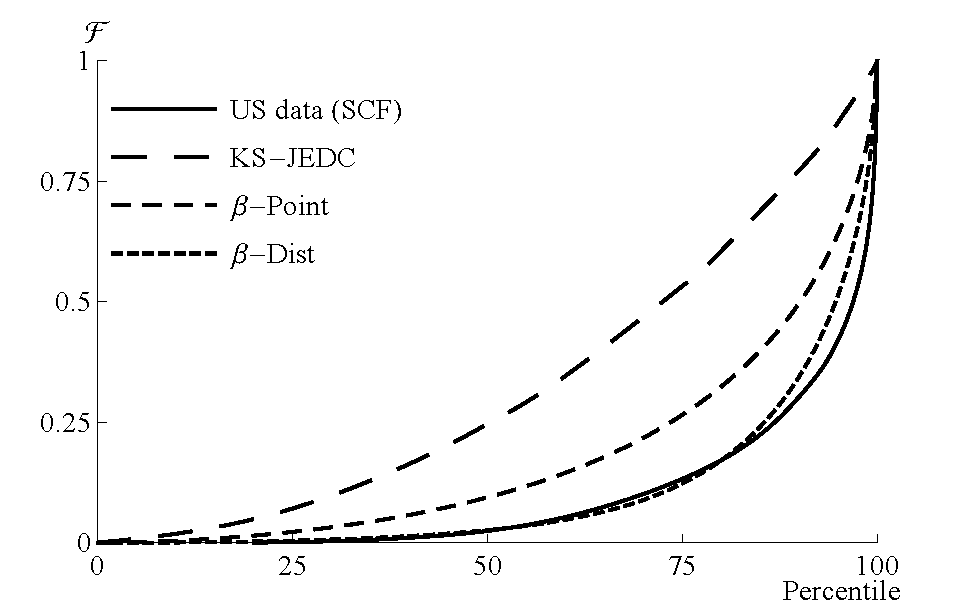
\includegraphics[width=0.9\textwidth]{../Figures/LifeCycleLorenzPlot.pdf}
%\caption{Cumulative Distribution of Net Worth}
\label{LifeCycleLorenzPlot}
\end{figure}

\end{frame}

\begin{frame}
\frametitle{{Results: MPC (in Annual Terms)}}
\begin{tiny}
\begin{table}
\input ../Tables/MPCslides_LCM.tex
\end{table}
\tiny{Notes: Annual MPC is calculated by $1-(1-$\text{quarterly MPC}$)^{4}$.
% See the paper for a discussion of the extensive literature that generally estimates empirical MPC's in the range of 0.3--0.6.
}
\end{tiny}
\end{frame}

\subsection{A Related Model}
\begin{frame}
\frametitle{Macro Handbook Model Like Ours, But With Multipliers}

`KMP': \cite{kmpHandbook}

Effect of mean-preserving spread in unemployment risk:

\begin{center}
\includegraphics[width=3in]{/Volumes/Sync/Dropbox/Bib/Raw/PDFs/kmpHandbook-Graphs/reseparately___/IRFCompareCextUIShockPropagationLong_1.pdf}
\end{center}

\end{frame}

\begin{frame}\frametitle{Other Results from KMP (Macro Handbook Paper)}

\begin{itemize}
\item Unemployment Insurance Has Big Macro Stabilization Role
\item Huge Heterogeneity in Cost of Business Cycles Across HH's
%\item Changes in Credit Availability Can Matter A Lot
\end{itemize}

\end{frame}

%\subsection{Conclusions}
%_______________________________________
\begin{frame}
\frametitle{Lessons}
\begin{itemize}
  \item Definition of ``serious'' microfoundations: Model that matches
\bi
\item Income Distribution and Income Dynamics
\item Wealth Distribution
\ei
  \item The model produces more plausible implications about:
  \bi
  \item \jemph{Aggregate MPC}
  \item \jemph{Distribution of MPC Across Households}
  \ei
  \item Can address questions like
\bi
\item Design of effective fiscal stimulus packages
\item How does conventional monetary policy work, and why
\item Which unconventional monetary policies will work
\item Role of Uncertainty in $C$ collapse
\item Macro stabilization consequences of unemployment insurance
\ei
\end{itemize}
\end{frame}

\section{Fiscal Policy}

\begin{frame}\frametitle{Larry Summers' Infamous Quote about 2009-10}

{\it ``Almost nothing from the academic macroeconomics literature over the prior
30 years was useful in understanding what to do''} 


\begin{center}
\phantom{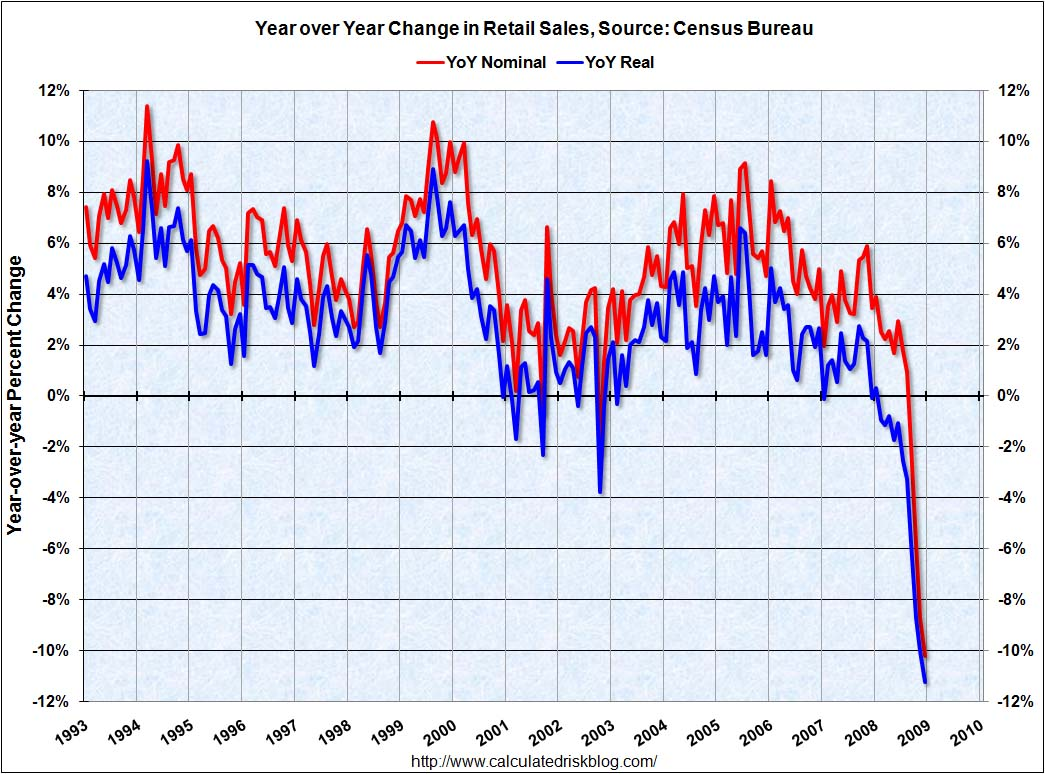
\includegraphics[width=2.5in]{/Volumes/Data/Job/Discuss/DiMaggio_Kermani/LaTeX/cfpbpresentation/Figures/Retail-Sales-Collapse.jpg}}
\end{center}

\end{frame}

\begin{frame}\frametitle{Larry Summers' Infamous Quote about 2009-10}

{\it ``Almost nothing from the academic macroeconomics literature over the prior
30 years was useful in understanding what to do''} 

\begin{center}
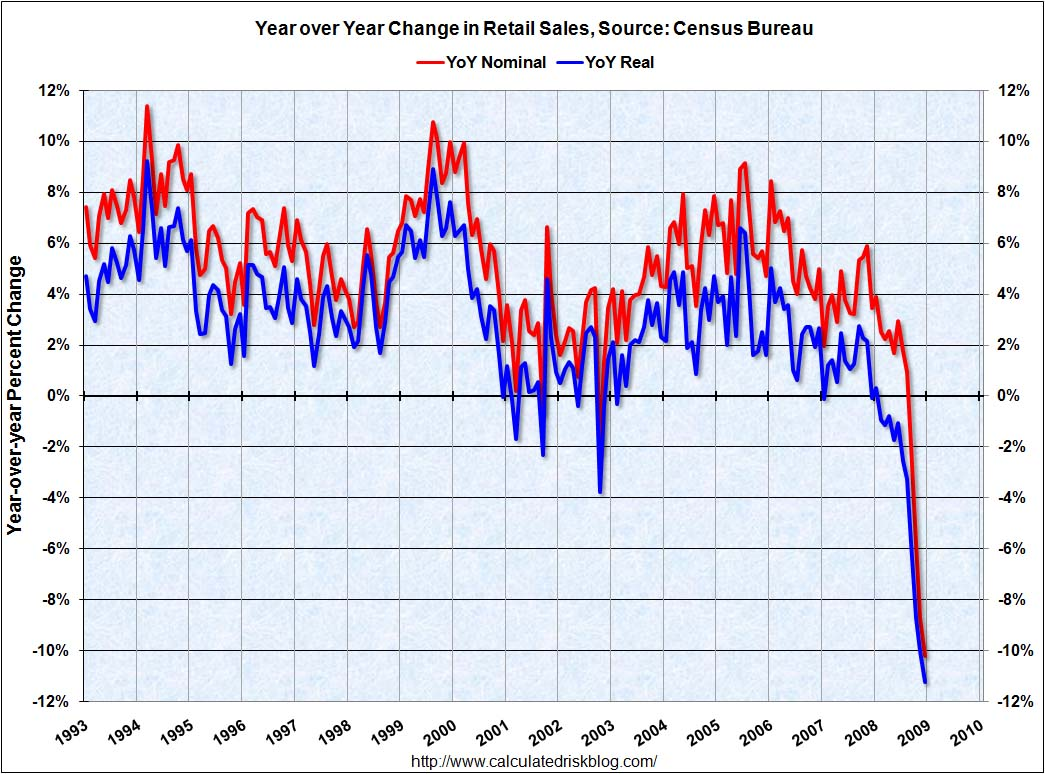
\includegraphics[width=2.5in]{/Volumes/Data/Job/Discuss/DiMaggio_Kermani/LaTeX/cfpbpresentation/Figures/Retail-Sales-Collapse.jpg}
\end{center}

\end{frame}

\begin{frame}\frametitle{What About Pre-1979 Macro?}

Keynesian \jemph{multipliers} should be big in liquidity trap \pause 

\medskip\medskip
Crudest Keynesian Model:
\begin{itemize}
\item $Y = C + I + G $ and $C = (Y-T) \MPC $
\begin{itemize}
\item Multipliers (if no pushback from monetary policy):
\begin{itemize}
\item G:~~1+$\MPC + \MPC^2 + \MPC^3 + ... = 1/(1-\MPC)$
\item T:~~\phantom{1+}$\MPC + \MPC^2 + \MPC^3 + ... =1/(1-\MPC)-1$
\end{itemize}
\end{itemize}

\begin{itemize}
\item If $\MPC = 0.75$ then multiplier on $G$ is 4 and $T$ is $4-1=3$
\bi
\item Recall: some micro estimates of $\MPC$ are this large
\ei
\item If $\MPC = 0.05$ then multiplier is only $\approx 0.05$
\bi
\item This is about the size of $\MPC$ in RA model without habits
\item RA models with habits, more like $\MPC=0.01$
\ei
\end{itemize}
\end{itemize}

\end{frame}

\begin{frame}\frametitle{Insights From HA Model + Pre-1978 Macro}


\begin{itemize}
\item `Stimulus' might be effective
\bi
\item Best kind would be $G$ spending
\item Want to target tax-based stimulus to high-MPC groups
\bi
\item Unemployed
\item Young
\item Low-Wealth
\ei
\item `Permanent'/persistent tax cuts more potent
\item Increase in uncertainty is a potential explanation of $C$ collapse
\ei
\end{itemize}

\end{frame}



\section{Monetary Policy}

\subsection{RANK}
\begin{frame}\frametitle{Money: Representative Agent New Keynesian Models}

\pause 
In RANK models, log-linearized Euler equation captures almost everything ($\sim$ 95 percent) of effect of 
monetary policy on $C$ dynamics:
\begin{eqnarray*}
  \Delta \log C_{t+1} & = & \CRRA^{-1}(\rfree_{t+1}-\timeRate)
\end{eqnarray*}

\pause 
Why?  When central bank makes $\rfree_{t+1}$ go up,
\begin{itemize}
\item People cut $C$ in order to take advantage of expected higher $r$
\end{itemize}

\pause 
Problems: \pause
\begin{itemize}
\item Essentially no evidence of {\it any} such sensitivity 
\item Log-linearization of Euler equation is a mathematical crime
\bi 
\item Not yet punishable by death ...   
\ei
\end{itemize}
\end{frame}

\subsection{HANK}


\begin{frame}
\frametitle{Heterogeneous Agent New Keynesian (HANK)} 

\begin{itemize}
\item Model like the one above plus New Keynesian prod fn
\end{itemize}
\end{frame}


\begin{frame}\frametitle{Monetary Policy According to HANK}

\cite{kmvHANK}

\medskip\medskip

\begin{itemize}
\item RANK IES channel accounts for only 15 percent of effect of $\rfree$
\item The rest reflects changes in income and wealth for groups with large $\MPC$
\bi
\item Debtors
\item Young People
\item Wealthy Hand-To-Mouth
\ei
\end{itemize}

\end{frame}

\subsection{Quantitative Easing}

\begin{frame}\frametitle{QE Works When It Affects High-MPC People}

\cite{dkpQE}:

QE1 worked and QE2 didn't because
\begin{itemize}
\item QE1 affected debtors (people with high MPC)
\item QE2 affected creditors (owners of Treasuries have a low MPC)
\item (and capital markets are segmented)
\end{itemize}


\end{frame}



\section{Uncertainty Over the Business Cycle}

\begin{frame}\frametitle{\cite{cssUSSaving}}
Structural model in which saving rate depends on:
\begin{itemize}
\item Household wealth
\item Credit Availability
\item Unemployment Expectations (as proxy for Uncertainty)
\end{itemize}

Results:

\begin{itemize}
\item Model estimated pre-2006 captures post-2006 $C$ collapse
\item In order of importance, model's explanation for $C$ collapse is:
\begin{enumerate}
\item Increase in uncertainty
\item Collapse in household wealth
\item Tightening of credit availability
\end{enumerate}
\end{itemize}

\end{frame}

\begin{frame}
\begin{center}
\centerline{Personal Saving Rate}

\includegraphics[width=2.5in]{/Volumes/Data/Papers/cssUSSaving/Latest/Figures/fPSR_StructFit.pdf}

\centerline{Red=Model; Black=Data}
\end{center}
\end{frame}

\section{\bf HARK!}

\begin{frame}\frametitle{Conclusion}

\begin{itemize}
\item {\it Benchmark} macro models need `serious' heterogeneity 
\begin{itemize}
\item It's not a `special case'
\end{itemize}
\item We know what to do 
\item Kernel of the technology is here:
\begin{itemize}
\item \href{http://econ-ark.org}{\texttt{http://econ-ark.org}}
\ifFRB{\item Come to next week's workshop to get started!}{}
\end{itemize}
\end{itemize}

\end{frame}

%_______________________________________
%\renewcommand{\bibsection}{\subsubsection*{\bibname }}

\nocite{denhaan:modelb}
\nocite{castaneda}


\beamerdefaultoverlayspecification{<*>}

\begin{frame}[t,allowframebreaks]
\frametitle{References}
\tiny 
\input econtexBibMake
\pagebreak

\end{frame}

\end{verbatimwrite}
\input ./HeteroMacro-Slides-body.tex


\end{document}
